


\section{Problem statement}
\label{sec:problem} 

The design and implementation of serious games synchronized with neurophysiological signals such as electroencephalography (EEG) presents a critical challenge, especially when targeting cognitive stimulation and diagnostic support in pediatric populations with Attention Deficit Hyperactivity Disorder (ADHD). The scientific validity of such applications is fundamentally dependent on the precise temporal synchronization of at least two disparate data streams: the high-temporal-resolution physiological data from the EEG system and the context-dependent event data generated by the serious game. A core technical obstacle lies in achieving this precise synchronization, a requirement that is essential for both the accuracy of event-related potential (ERP) measurements and the effectiveness of real-time interventions.1 This thesis addresses two primary facets of this challenge: the temporal inaccuracies introduced by system-level operations and the physical limitations of the hardware itself.

\subsection{Unpredictable Latency and Jitter Between Game Events and EEG Recordings}

The primary technical issue in synchronizing EEG data with serious game events is the presence of unpredictable latency and jitter.2
Latency is the delay between an event's physical occurrence (e.g., a stimulus appearing on screen) and its corresponding timestamp being recorded in the data stream. A more pernicious issue is jitter, defined as the statistical variability in that latency over time.4 While a constant latency might be correctable in post-processing, jitter introduces random, unpredictable timing errors that cannot be easily removed after data acquisition.
This issue is caused by several interrelated factors: buffering delays in data pipelines, the non-deterministic scheduling of non-real-time operating systems, variability in communication protocols (such as USB, Bluetooth, or the Lab Streaming Layer), and asynchronous execution within game engines like Unity.5 These conditions lead to a lack of temporal precision, where the timestamp of an in-game event does not accurately align with the corresponding entry in the EEG data stream.
This misalignment significantly compromises the quality of neurophysiological analysis. ERP components such as the P300 and N200, which are commonly used to evaluate attentional processes in ADHD, depend on millisecond-level synchronization between stimulus onset and neural response.7 When event markers are not precisely aligned due to jitter, the resulting ERP waveform becomes temporally "smeared," causing a reduction in both amplitude and interpretability, which degrades the signal-to-noise ratio and threatens diagnostic reliability.2 This is particularly critical in pediatric populations where subtle attentional deficits are being assessed.
Furthermore, in real-time systems like neurofeedback applications, where immediate feedback is essential for operant conditioning, even minor delays can disrupt the feedback loop. If the user receives auditory or visual feedback that no longer corresponds precisely to their brain state, the therapeutic effectiveness is reduced, potentially leading to user disengagement or ineffective training outcomes.2 The temporal precision required is demanding; some brain-computer interface (BCI) paradigms require accuracy within ±2 milliseconds, yet jitter introduced by a game's graphical rendering at 50 frames per second can be as high as 20 milliseconds.
Recent studies have quantified these challenges. For example, Larsen et al. (2024) found that even in systems optimized with Unity and LSL, event marker delays averaged 36 milliseconds with a jitter of 5 to 6 milliseconds—well above the acceptable margin for many ERP analyses.9 Additionally, Brain Products (2024) reports that embedded platforms lacking efficient buffering and timestamping can exhibit latencies up to 100 milliseconds, particularly under high computational load.5 These delays, caused by a lack of dedicated real-time scheduling and protocol optimization, result in a substantial loss of synchronization fidelity, ultimately undermining both research validity and clinical utility.


\subsection{Resource and power constraints in embedded EEG platforms}

The second major issue stems from the computational and energy limitations of embedded and wearable EEG systems. Designed to be mobile and unobtrusive, these systems often operate on limited battery power, constrained CPU cycles, and reduced memory.11 These constraints are exacerbated when the system must simultaneously support real-time data acquisition, multichannel EEG streaming, and high-frequency event marker registration. Conventional EEG setups that rely on centralized data processing can also lead to high energy consumption and increased data transmission latency.12
These limitations make it difficult to implement low-latency communication and high-resolution timestamping. Wireless data transmission, in particular, is very power-intensive.13 Protocols such as Bluetooth and Wi-Fi—commonly used in portable EEG systems—can introduce packet retransmissions, buffering delays, and inconsistent delivery times that worsen synchronization accuracy.5
The consequences are significant. System designers are forced to lower EEG sampling rates, simplify marker handling, or accept increased delays—all of which reduce the reliability of the collected data and the interactivity of the game.14 For example, a review of wearable EEG systems found that wireless devices consistently showed worse timing stability and synchronization performance compared to wired configurations, especially when embedded resources were under heavy computational load.
Brain Products (2024) corroborates these findings, warning that system performance degrades as channel count and sampling rate increase—conditions commonly required in clinical-grade EEG systems.5 This creates a fundamental trade-off: increasing signal fidelity and temporal resolution compromises system portability, while optimizing for mobility sacrifices diagnostic precision.
Therefore, a critical gap exists in establishing a robust methodology to reliably synchronize multimodal data streams from EEG systems and dynamic serious games with quantifiable, millisecond-level precision, while also operating within the power and resource constraints of embedded platforms. This thesis addresses the problem of ensuring the temporal integrity of these data streams to enable scientifically valid analysis of neuro-cognitive processes during gameplay.


%The design and implementation of serious games synchronized with neurophysiological signals such as EEG presents a critical challenge in the domain of embedded systems, especially when targeting cognitive stimulation and diagnostic support in pediatric populations with Attention Deficit Hyperactivity Disorder (ADHD). A core technical obstacle lies in achieving precise synchronization between in-game events and EEG signal acquisition, a requirement that is essential for both the accuracy of event-related potential (ERP) measurements and the effectiveness of real-time interventions.

% \section{Problem Statement}

% The integration of EEG acquisition systems with serious games for neurocognitive stimulation and ADHD diagnosis in children is gaining relevance due to its potential for real-time, objective assessment of brain activity. However, when such systems are deployed on embedded or mobile platforms, two critical technical challenges arise that compromise their effectiveness: (1) unpredictable latency and jitter between the game engine and the EEG recorder, and (2) the resource and power constraints inherent to embedded systems. Both issues severely affect the temporal precision required for capturing event-related potentials (ERPs) and delivering valid neurofeedback or cognitive training.

%\subsection{Unpredictable Latency and Jitter Between Game Events and EEG Recordings}

%One of the primary technical issues in synchronizing EEG data with serious game events is the presence of unpredictable latency and jitter during the transmission of event markers. This issue is caused by several interrelated factors: buffering delays in data pipelines, the non-deterministic scheduling of non-real-time operating systems, variability in communication protocols (such as USB CDC, Bluetooth, or Lab Streaming Layer), and asynchronous execution within game engines like Unity. These conditions lead to a lack of temporal precision, where the timestamp of an in-game event does not accurately align with the corresponding entry in the EEG data stream.

%As a consequence, this misalignment significantly compromises the quality of neurophysiological analysis. ERP components such as the P300 and N200, commonly used to evaluate attentional processes in ADHD, depend on millisecond-level synchronization between stimulus onset and neural response. When event markers are not precisely aligned due to jitter or latency, the resulting ERP waveform becomes temporally smeared, causing a reduction in both amplitude and interpretability \cite{iwama2022jitter}. This degradation affects diagnostic reliability, particularly in pediatric populations where subtle attentional deficits are being assessed.

%Another cause of latency variability stems from the processing demands of real-time systems. In neurofeedback applications, where immediate feedback is essential for operant conditioning, even minor delays in EEG–event synchronization can disrupt the feedback loop. As a consequence, the user receives auditory or visual feedback that no longer corresponds precisely to their brain state, thereby reducing the therapeutic effectiveness and potentially leading to user disengagement or ineffective training outcomes.

%Recent studies have further demonstrated the impact of these technical challenges. For example, \cite{larsen2024quantifying} found that even in systems optimized with Unity and LSL, event marker delays averaged 36 milliseconds, with jitter ranging from 5 to 6 milliseconds—well above the acceptable margin for ERP-based analyses. Additionally, \cite{brainproducts2024lsl} reports that embedded platforms lacking efficient buffering and timestamping mechanisms can exhibit latencies up to 100 milliseconds, particularly under high computational load or poorly configured data streams. These delays are caused by a lack of dedicated real-time scheduling and protocol optimization, and the resulting consequence is a substantial loss of synchronization fidelity—ultimately undermining both research validity and clinical utility.


%\subsection{Resource and power constraints in embedded EEG platforms}

%The second major issue stems from the computational and energy limitations typical of embedded EEG systems. These systems, designed to be mobile and unobtrusive, often operate on limited battery power, constrained CPU cycles, reduced memory, and variable wireless connectivity. These constraints are exacerbated when the system must support real-time data acquisition, multichannel EEG streaming, and high-frequency marker registration simultaneously.

%These limitations make it difficult to implement low-latency communication and high-resolution timestamping. In particular, wireless protocols such as Bluetooth and Wi-Fi—commonly used in portable EEG systems—introduce packet retransmissions, buffering delays, and inconsistent delivery times that worsen synchronization accuracy.

%The consequences are significant. System designers are forced to lower EEG sampling rates, simplify marker handling, or accept increased delays—all of which reduce the reliability of the collected data and the interactivity of the game. For example, \cite{liu2024fpga} reviewed wearable EEG systems and found that wireless devices consistently showed worse timing stability and synchronization performance compared to wired configurations, especially when embedded resources were under heavy computational load.

%\cite{brainproducts2024lsl} corroborates these findings, warning that system performance degrades as channel count and sampling rate increase—conditions commonly required in clinical-grade EEG systems. This creates a fundamental trade-off: increasing signal fidelity and temporal resolution compromises system portability, while optimizing for mobility sacrifices diagnostic precision.

\begin{figure}
    \centering
    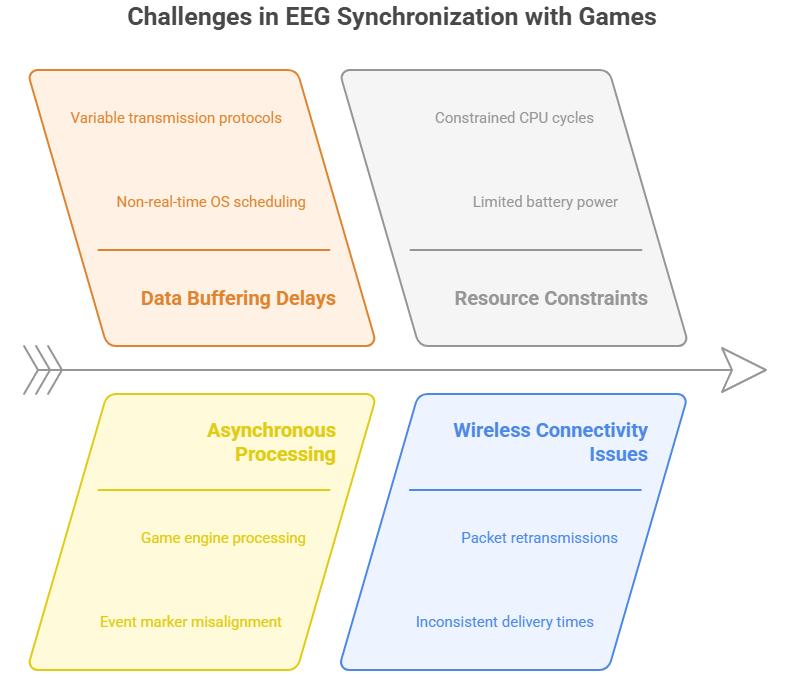
\includegraphics[width=0.8\linewidth]{Cap 1/Figures/state of the art.png}
    \caption{}
    \label{fig:Esquema}
\end{figure}

% In summary, the combined effects of latency/jitter and resource limitations in embedded EEG systems threaten the temporal accuracy and clinical reliability of serious games for ADHD evaluation. These challenges must be addressed to ensure that event markers in the game are precisely aligned with EEG recordings, and that the system can operate effectively in real-world, mobile, and child-friendly environments.





% \subsection{Lattency and jitter}

% One major subproblem is the presence of latency and jitter in the transmission of event markers from the game engine to the EEG recording system. Even under tightly controlled experimental setups, delays in marker delivery can vary significantly due to factors such as USB buffering, wireless transmission, and operating system scheduling. Recent studies report latency offsets averaging 36 ms with jitter exceeding 5 ms in Unity–LSL pipelines, which can distort ERP measurements and limit the effectiveness of closed-loop systems (Larsen et al., 2024). Moreover, Iwama et al. (2022) emphasize that even small jitters of ±5 ms are sufficient to degrade the temporal accuracy required for neurofeedback and ERP-based paradigms. Vendor documentation from Brain Products (2024) warns that such delays can reach up to 100 ms on low-power embedded devices unless buffering and sampling rates are carefully tuned.

% % \subsection{synchronization interface}

% % A second subproblem is the lack of standardized synchronization interfaces across the heterogeneous hardware and software components involved in EEG–game integration. Serious games, microcontrollers, and EEG amplifiers often utilize disparate protocols such as TTL pulses, USB CDC, BLE, and Lab Streaming Layer (LSL), each with its own timing architecture and limitations. Miziara et al. (2025) found that hardware-based triggers offered substantially greater timing accuracy than software-based LSL alternatives, though at the expense of system scalability. Similarly, commercial EEG systems such as Zeto WR19 can embed low-jitter markers via proprietary hardware, but still require complex reconciliation when integrating third-party devices through LSL or TTL (Zeto Inc., 2023). Brain Products (2024) highlights the risk of marker misalignment when synchronizing systems that rely on different timestamping strategies without a unified clock.

% \subsection{Resource and power constraints in mobile/embedded EEG platforms}


% A third subproblem arises from computational and power limitations in mobile or embedded EEG systems, which restrict the feasibility of implementing high-resolution, low-latency synchronization protocols. Mobile EEG devices often operate on limited battery capacity and rely on wireless communication, which introduces variable delays due to packet buffering and retransmission. Liu et al. (2024) observed that wireless EEG systems generally exhibit reduced temporal stability compared to their wired counterparts, especially under higher sampling rates or increased channel counts. Brain Products (2024) also notes that latency tends to increase with system load, further complicating efforts to achieve precise synchronization in portable scenarios.
% These synchronization challenges are particularly consequential in ADHD-focused applications, where the reliability of stimulus-locked EEG features such as the P300 or N200 components is crucial for diagnostic and therapeutic efficacy. Real-time adaptive feedback mechanisms—common in gamified neurofeedback interventions—require consistent round-trip latencies under 100 ms, while embedded systems deployed in schools or clinics must balance timing accuracy with constraints on power, cost, and usability. Addressing the issues of latency and jitter, protocol standardization, and resource optimization is thus vital for the development of robust and clinically useful EEG–game synchronization systems.


% Agregar las graficas del estado del arte 


\newpage
\section{Pregunta de investigación}\label{sec:question}

How can a low-latency and low-jitter data synchronization framework be developed and validated to ensure the temporal integrity of multimodal data from embedded EEG systems and dynamic serious game events, while respecting the inherent resource and power constraints of such platforms?


